

\tikzset{every picture/.style={line width=0.75pt}} %set default line width to 0.75pt        

\begin{tikzpicture}[x=0.75pt,y=0.75pt,yscale=-1,xscale=1]
	%uncomment if require: \path (0,294); %set diagram left start at 0, and has height of 294
	
	%Image [id:dp6050577265750149] 
	\draw (256.6,91.52) node  {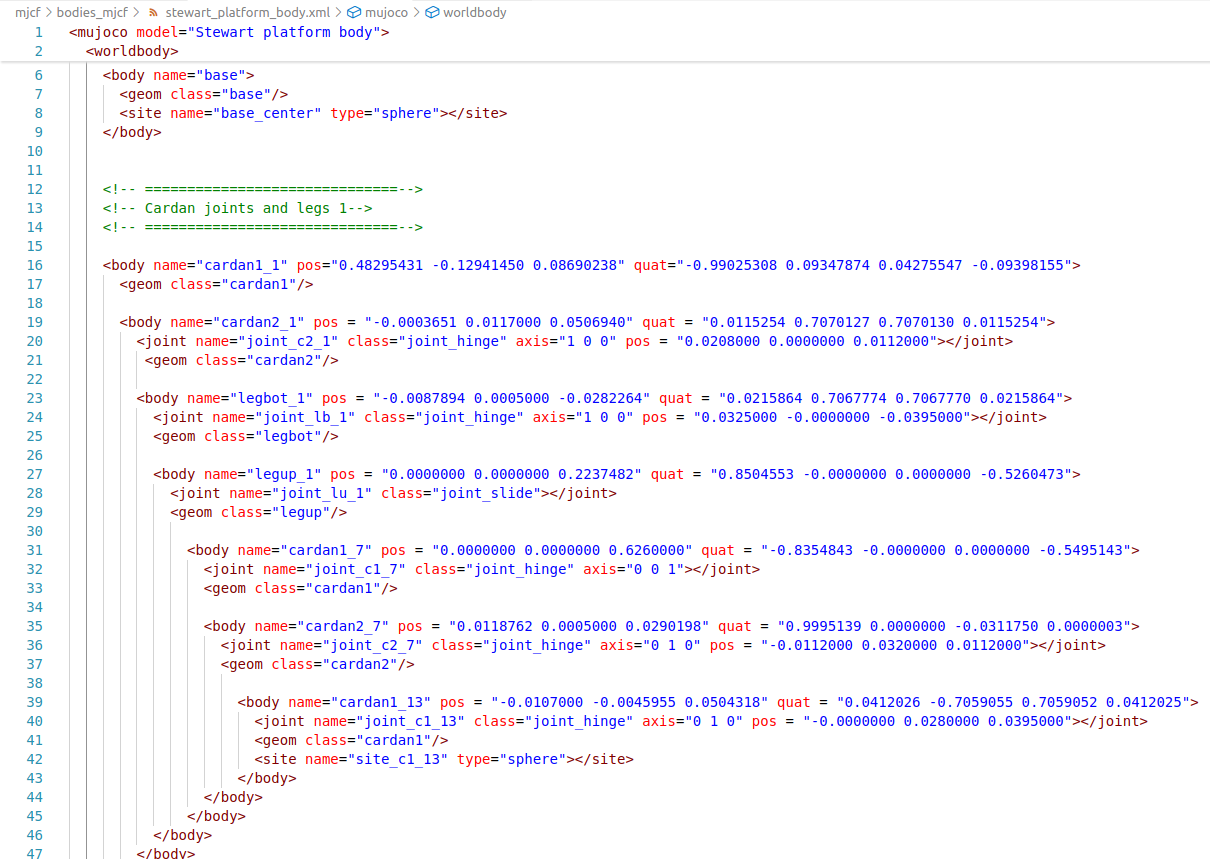
\includegraphics[width=113.4pt,height=74.88pt]{vscode-xml.png}};
	%Image [id:dp4103408524493818] 
	\draw (301.67,56.56) node  {
\includegraphics[width=18.91pt,height=17.59pt]{gg-xml.png}};
	%Shape: Rectangle [id:dp16081927472626079] 
	\draw   (181,41.6) -- (332.2,41.6) -- (332.2,141.44) -- (181,141.44) -- cycle ;
	
	%Image [id:dp9369943974675126] 
	\draw (82.6,144.7) node  {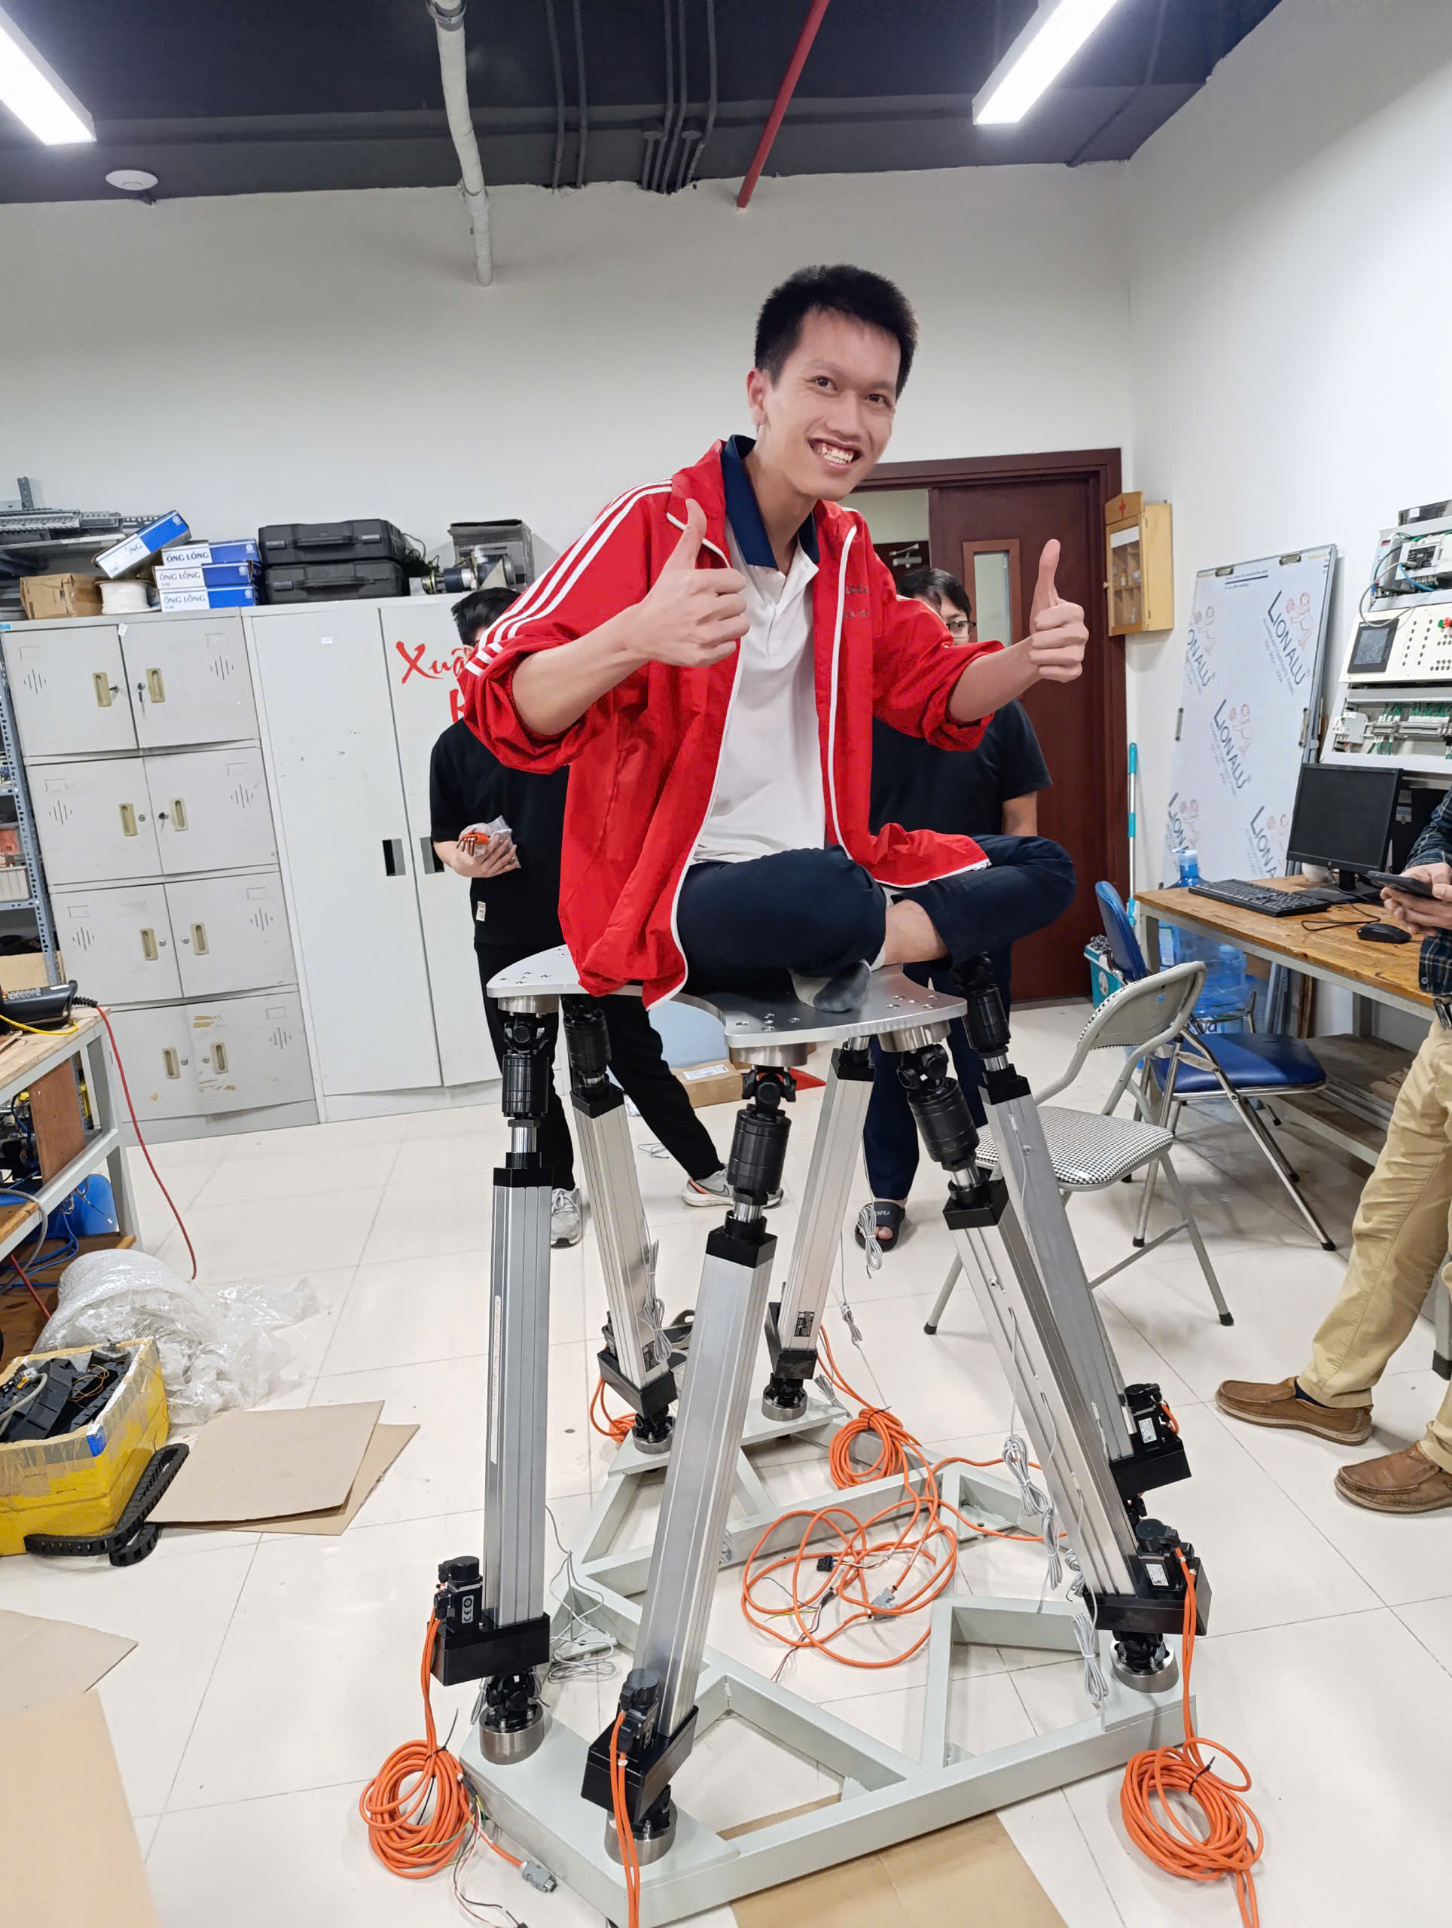
\includegraphics[width=95.4pt,height=126.15pt]{real-stewart.png}};
	%Shape: Rectangle [id:dp929363304432309] 
	\draw   (19,60.6) -- (146.2,60.6) -- (146.2,228.8) -- (19,228.8) -- cycle ;
	
	%Image [id:dp5416117995243275] 
	\draw (521.1,109.06) node  {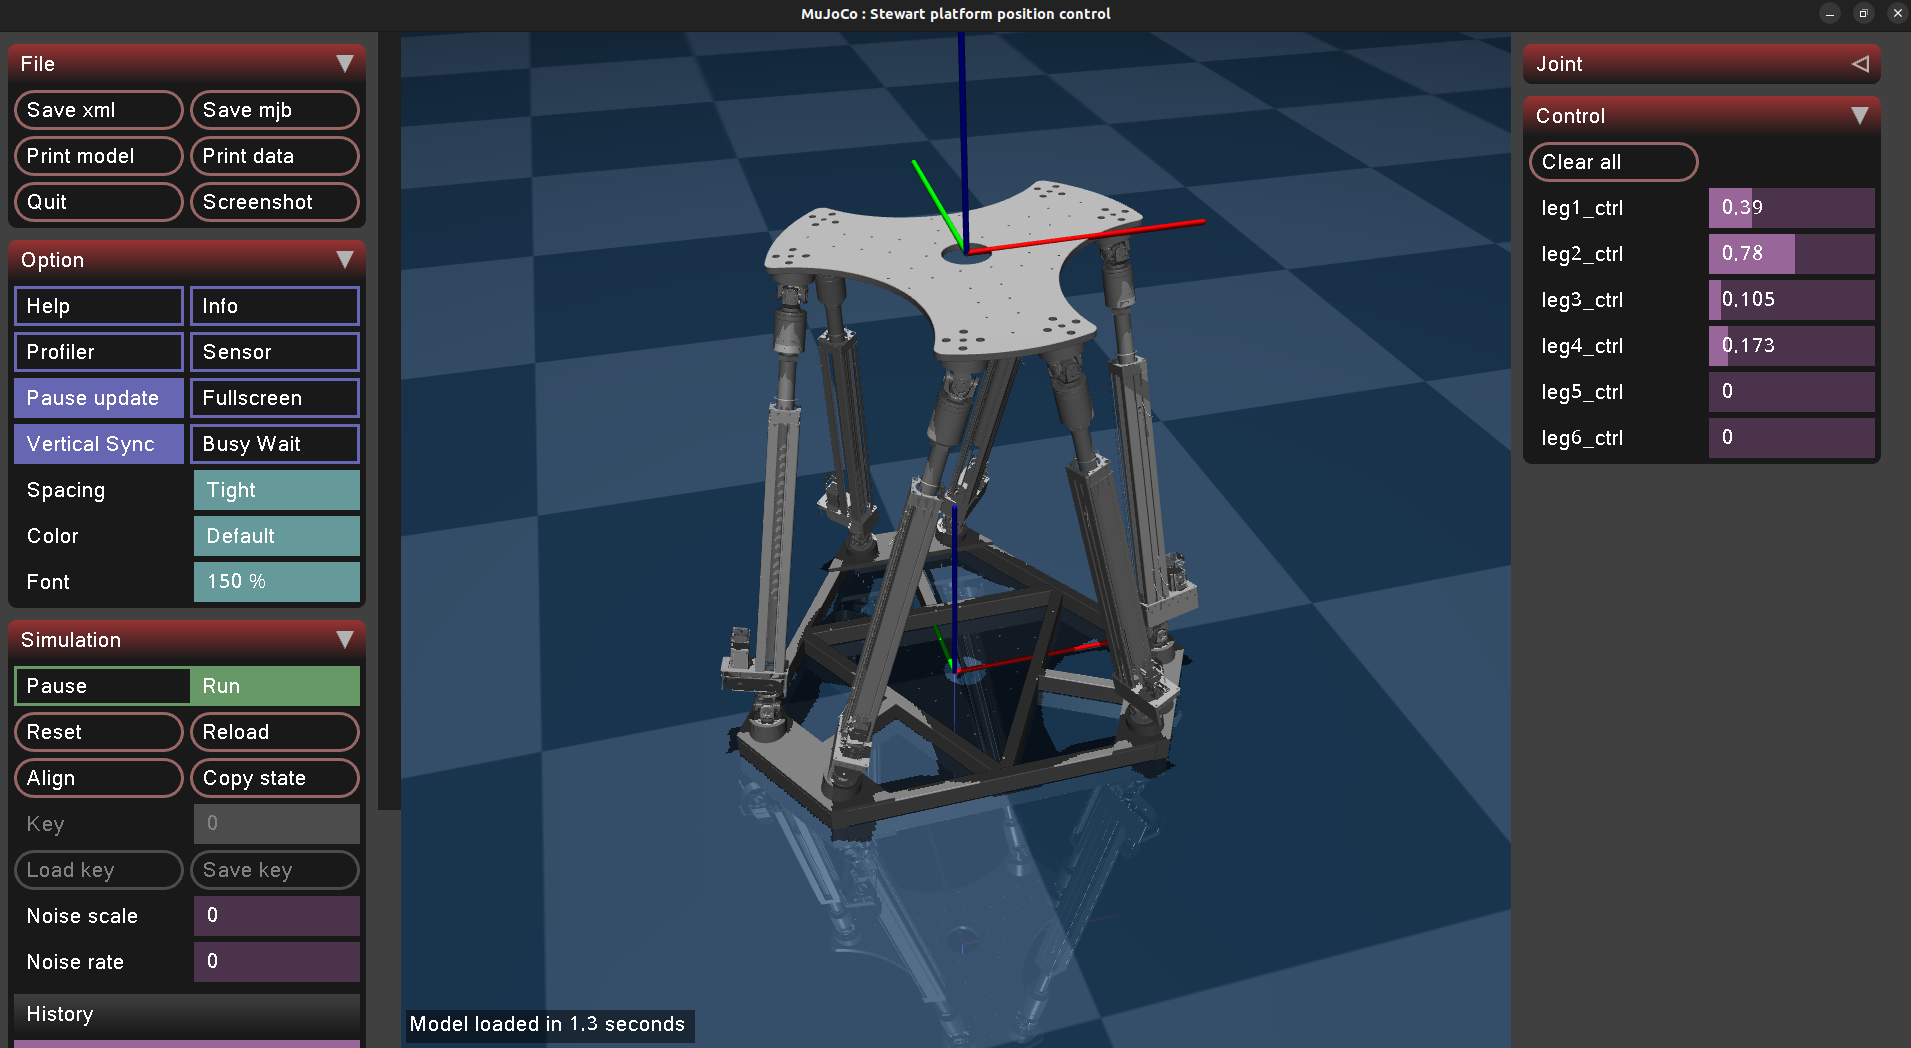
\includegraphics[width=186.15pt,height=102.09pt]{mujoco-stewart.png}};
	%Shape: Rectangle [id:dp0001749169919830207] 
	\draw   (397,41) -- (645.2,41) -- (645.2,177.11) -- (397,177.11) -- cycle ;
	
	%Rounded Rect [id:dp5884670081331446] 
	\draw   (8.2,32.6) .. controls (8.2,19.9) and (18.5,9.6) .. (31.2,9.6) -- (337.2,9.6) .. controls (349.9,9.6) and (360.2,19.9) .. (360.2,32.6) -- (360.2,256.6) .. controls (360.2,269.3) and (349.9,279.6) .. (337.2,279.6) -- (31.2,279.6) .. controls (18.5,279.6) and (8.2,269.3) .. (8.2,256.6) -- cycle ;
	%Bend Up Arrow [id:dp4779894085615144] 
	\draw   (380,254.96) -- (519.1,254.96) -- (519.1,219.02) -- (511.04,219.02) -- (525.12,199.6) -- (539.2,219.02) -- (531.14,219.02) -- (531.14,267) -- (380,267) -- cycle ;
	%Image [id:dp23296886516718363] 
	\draw (256.1,203.11) node  {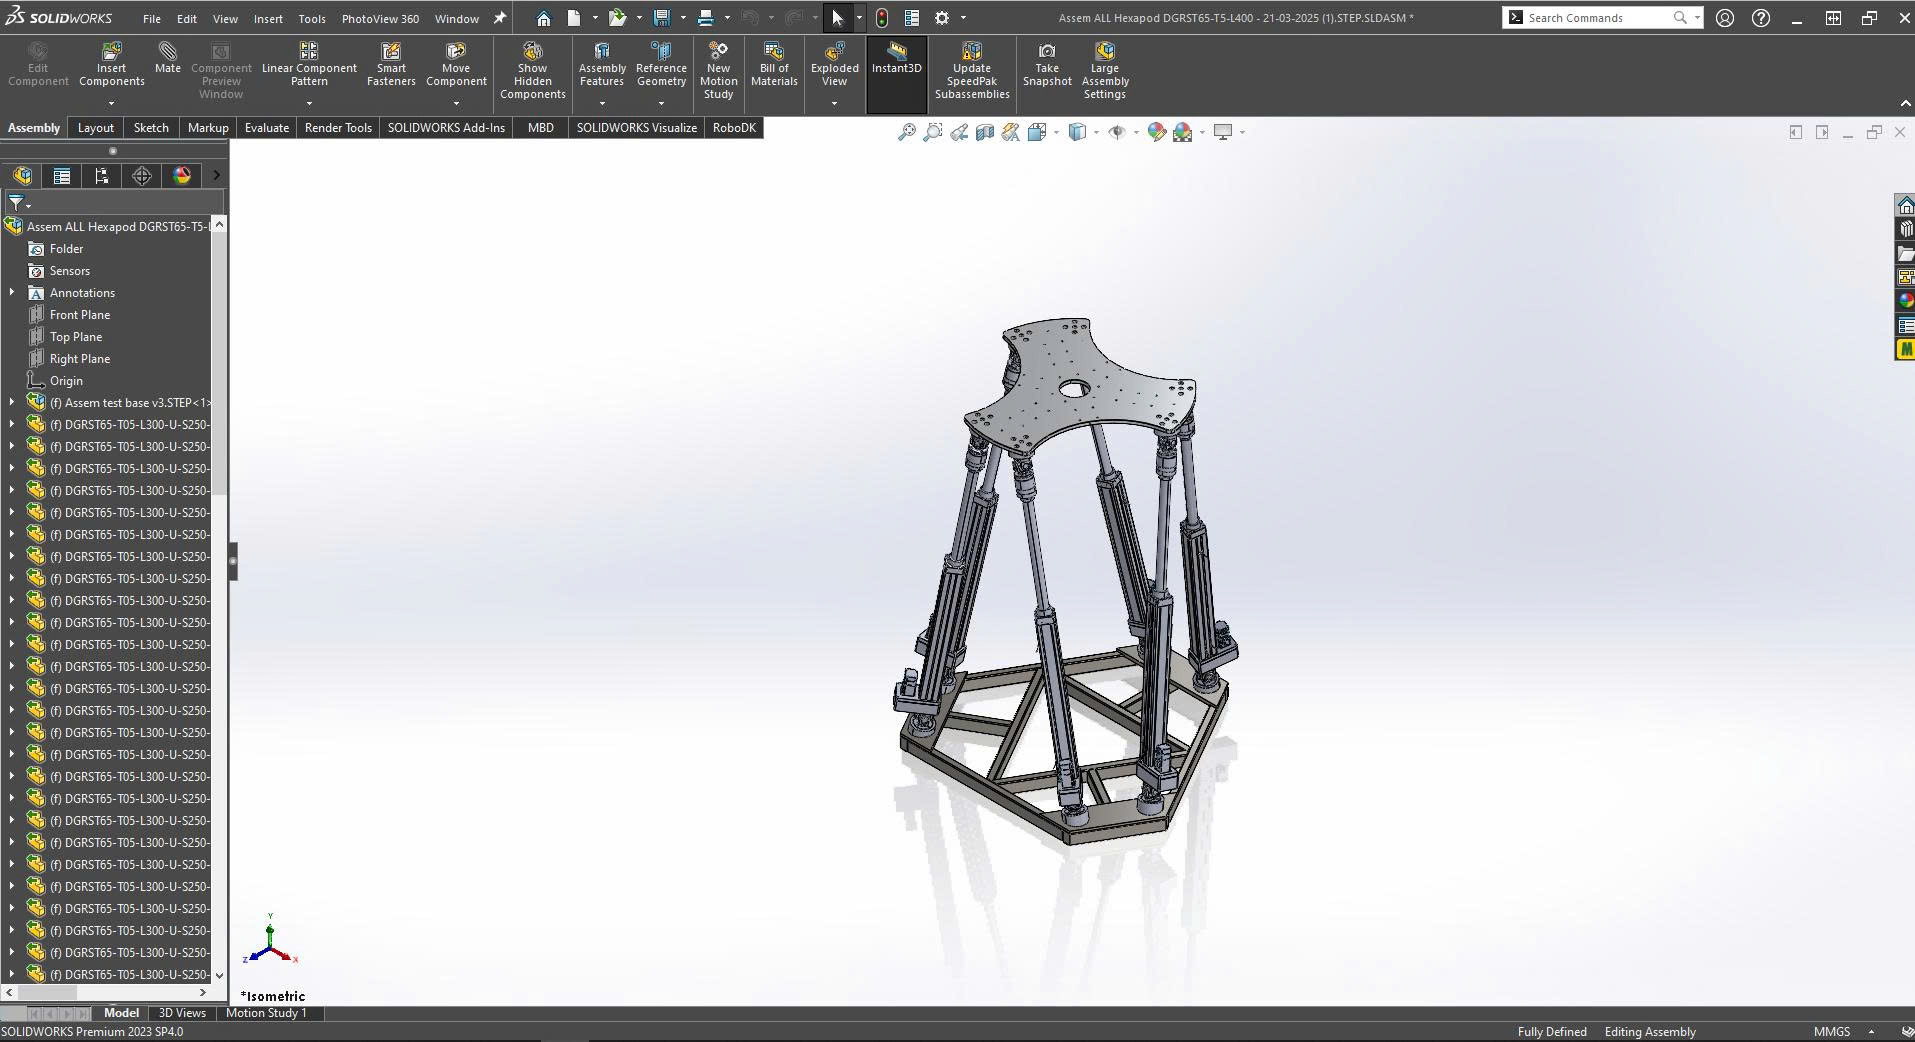
\includegraphics[width=138.15pt,height=75.17pt]{sw-stewart.jpg}};
	%Shape: Rectangle [id:dp47379488924670254] 
	\draw   (164,153) -- (348.2,153) -- (348.2,253.23) -- (164,253.23) -- cycle ;
	
	
	% Text Node
	\draw (183,38.6) node [anchor=south west] [inner sep=0.75pt]   [align=left] {xml descriptions};
	% Text Node
	\draw (166,256.23) node [anchor=north west][inner sep=0.75pt]   [align=left] {computer aided design};
	% Text Node
	\draw (21,231.8) node [anchor=north west][inner sep=0.75pt]   [align=left] {real-world model};
	% Text Node
	\draw (399,38) node [anchor=south west] [inner sep=0.75pt]   [align=left] {MuJoCo model};
	
	
\end{tikzpicture}
